\documentclass[11pt,letterpaper]{article}
\usepackage{fullpage}
\usepackage{multicol}
\usepackage{amsmath}
\usepackage{amsfonts}
\usepackage{amssymb}
%\usepackage{pstricks, pst-node, pst-plot}

\ifx\pdfoutput\undefined
% we are running LaTeX, not pdflatex
\usepackage{graphicx}
\else
% we are running pdflatex, so convert .eps files to .pdf
\usepackage[pdftex]{graphicx}
\usepackage{epstopdf}
\fi

\newcommand{\ds}{\displaystyle}
\newcommand{\bv}{\mathbf}
\newcommand{\lv}{\langle}
\newcommand{\rv}{\rangle}

\begin{document}
\flushleft
\begin{multicols}{2}

\begin{large}\textbf{Math 116 Quiz 5: $\oint$ 11.1-11.6 (Differential Equations) \\
Tue 23 Oct 2012}\end{large}

\textbf{Name:  }\underline{\hspace{35ex}}

\vspace{.5in}

\end{multicols}

\pagestyle{empty}


\flushleft

You have 30 minutes to complete this quiz.  Eyes on your own paper and good luck!

\begin{enumerate}
\item  \textbf{Definitions/Concepts.} (1 pt ea) Consider a differential equation of the form
\[\frac{dH}{dt}=k(H-C),\]
where $k$ and $C$ are constants.
\begin{enumerate}
\item This is a \underline{\hspace{10ex}} order differential equation.

\vspace{1pc}
\item What is the general solution to this equation?

\vspace{10pc}
\item What is the equilibrium solution to this equation?

\vspace{4pc}
\end{enumerate}
 
\item \textbf{Questions/Problems.} 

A box is dropped from an airplane.  The downward veleocity $v(t)$ of the box, once its parachute opens, satisfies the differential euqation
\[\frac{dv}{dt}=10-\frac{1}{10}(1+e^{-t})v^2.\]
\begin{enumerate}
\item (3 pts)
Suppose the parachute opens when the velocity of the box is 11 m/s.  Use Euler's method with three steps to approximate the velocity of the box one second after the parachute opens.
\[\begin{array}{|c|c|c|c|}
\hline
t & v(t) & dv/dt & \Delta v \\ [0.5ex]
\hline 
\hspace{10ex} & \hspace{10ex} & \hspace{10ex} & \hspace{10ex} \\ [0.5ex]
\hline
\hspace{10ex} & \hspace{10ex} & \hspace{10ex} & \hspace{10ex} \\ [0.5ex]
\hline 
\hspace{10ex} & \hspace{10ex} & \hspace{10ex} & \hspace{10ex} \\ [0.5ex]
\hline
\end{array}\]

What does your estimate say the velocity is after 1 second?

\vspace{3pc}
\hfill{\bf MORE QUIZ ON THE BACK --\textgreater}

\item (2 pts) Draw your Euler approximation on the following slope field:
\smallskip
\begin{center}
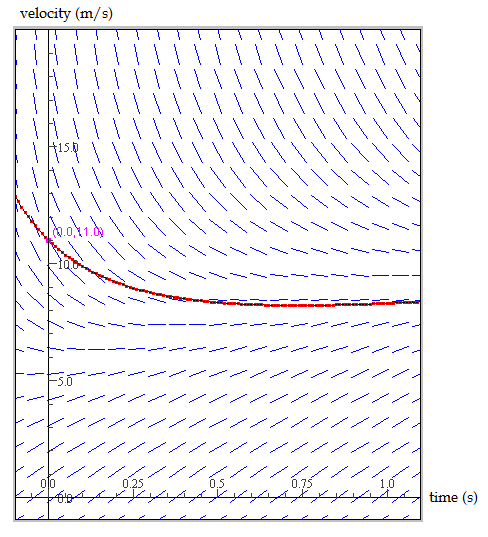
\includegraphics{quiz5slfld.png}
\end{center}

\item (2 pts) Say something {\bf about slope fields} to argue whether your approximation is an overestimate or an underestimate.

\vspace{3pc}
\end{enumerate}

\item \textbf{Computations/Algebra.} (1 pt ea) Find the solutions to the following differential equations subject to their given initial conditions.
\begin{enumerate}
\item $\frac{dy}{dx}+\frac{y}{3}=0,\;\;y(0)=10$

\vspace{10pc}
\item $2\frac{du}{dt}=u^2,\;\;u(0)=1$

\vspace{10pc}
\item $\frac{dz}{dy}=zy,\;\;z=1\text{ when }y=0$

\vspace{10pc}
\item $\frac{dz}{dt}=te^z,\;\;\text{ through the origin}$

\vspace{10pc}
\item $\frac{dw}{d\theta}=w+w\theta^2,\,\,w=5\text{ when }\theta=0$

\end{enumerate}

\end{enumerate}

\end{document}


